\section{Algorithmic Ideas and Implementation}
\label{algorithms}
This section discusses the key algorithmic ideas implemented in EASAL. EASAL
starts by generating all possible active constraint graphs with 1 or 2
(depending on user input) active constraints yielding 5D or 4D regions
(represented as root nodes) in the atlas and then successively samples them.
The main algorithm, ALGORITHM \ref{alg:sampleAtlasNode} merges the three
strategies described in the previous section.

\begin{algorithm} [htbp]
 \SetKwInOut{Input}{input}\SetKwInOut{Output}{output}

 {\bf sampleAtlasNode}\\
 \Input{atlasNode: node}
 \Output{Complete sampling of the atlasNode and all its children}
 \BlankLine

	$H$ = node.activeConstraints\\
	$G_H$ = node.activeConstraintGraph\\
	\If{ $G_H$ is minimally rigid}
		{stop;	}
	$F$ = complete3Tree($G_H$)\\
	
	$C$ = computeConvexChart($G_H$, $F$)\\

	\For{ each cayleyPoint $p$ within convexChart $C$ }
	{
		$R$ = computeRealizations($p$)\\

		\For{ each realization $r$ in $R$}
		{
			\If{!aPosterioriConstraintViolated($r$)}
			{
				\If{ isBoundaryPoint($r$) \&\& hasNewActiveConstraint($r$, $G_H$) }
				{
					$e$ = newActiveConstraint($r$, $G_H$);\\
					$G'$ := $G_{H \cup \{e\}}$ ;\\
					\If{ $G'$ is not already present in the current atlas}
					{
						childNode = new atlasNode($G'$)\\
						childNode.insertWitness($p$);\\
						sampleAtlasNode(childNode);\\
					} \Else{
						childNode = findNode($G'$);
					}
					node.setChildNode(childNode);
				} 
			}
		}
	}
	\caption{High level EASAL pseudocode}
\label{alg:sampleAtlasNode}
\end{algorithm}


ALGORITHM \ref{alg:sampleAtlasNode} proceeds as follows. It (i) recursively
(by depth first search) generates the atlas by discovering active constraint
regions of decreasing dimension; (ii) uses Cayley convexification of the region
to efficiently compute bounds for Cayley parameters a priori (before
realization), and samples Cayley configurations in this convex region; (iii)
detects boundary regions of 1 dimension less a posteriori (after realization)
i.e., when a new constraint becomes active, and efficiently finds the (finitely
many) Cartesian realizations of the Cayley configuration samples. We describe
each of these aspects of the algorithm in Sections \ref{sec:exploration},
\ref{sec:tetrahedralbounds} and \ref{sec:boundarydetection} respectively.

\subsection{Atlasing and Stratification}
\label{sec:exploration}
EASAL stores and labels regions of the Cartesian configuration space as an
atlas as described in Section \ref{sec:stratification}. The regions of the
atlas are stored as nodes of a directed acyclic graph, whose edges represent
boundary relationships. Each region of the atlas is an active constraint region
associated with a unique active constraint graph $G_H$, where $H$ is the set of
active constraints (see Algorithm 1). 

The exploration of the atlas is done by the recursive \textbf{sampleAtlasNode}
algorithm using one of the generated atlas root nodes as input. Using depth
first search, this algorithm samples the atlas node and all its descendants.
\figref{fig:algorithm} gives an overview of the algorithm.


\begin{figure}
\centering
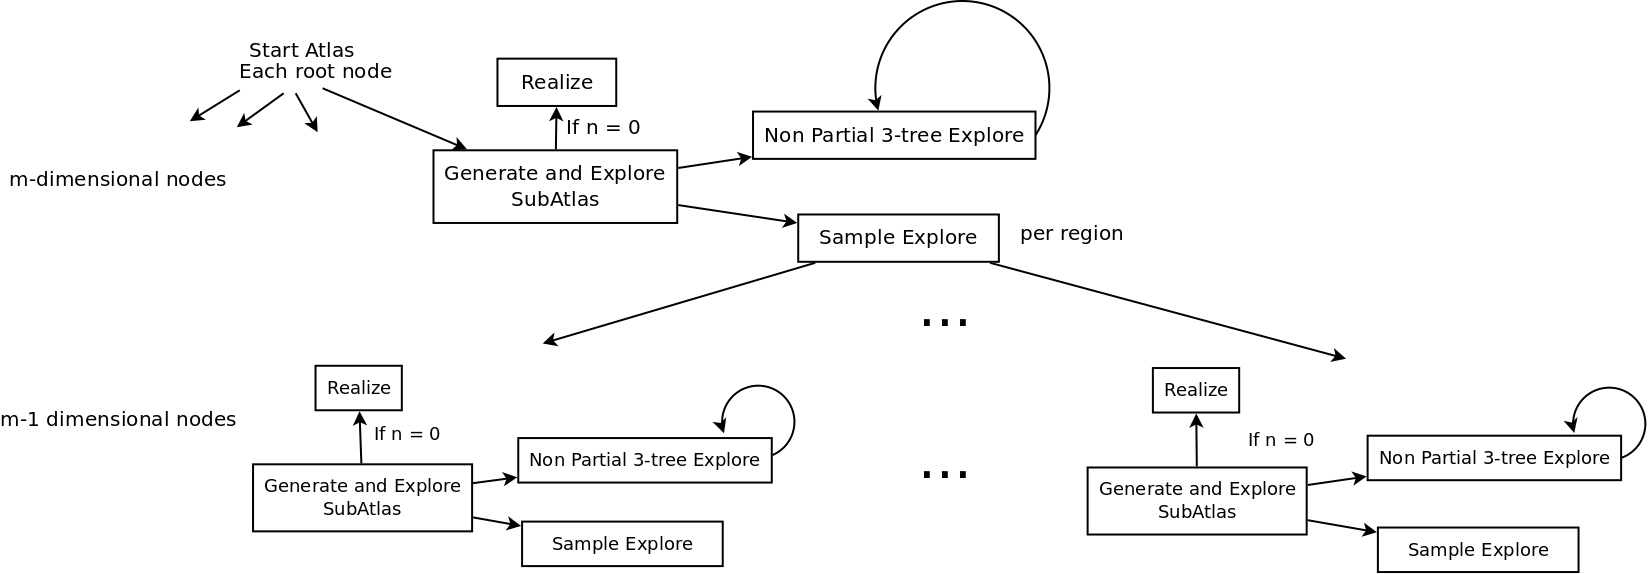
\includegraphics[width=\textwidth] {\fig/Algorithm.png}
\caption{A high level flowchart of the algorithm for generating and exploring the atlas}
\label{fig:algorithm}
\end{figure}


\noindent\textbf{Base case of recursion:} If active constraint graph $G_H$ of
the node is minimally rigid i.e., the active constraint region is 0D, then
there is only 1 Cayley configuration (with finitely many Cartesian
realizations).  We have no more sampling to do, hence return.

\noindent\textbf{The recursion step:} If $G_H$ is not minimally rigid, EASAL
applies the \textbf{complete3Tree} algorithm of in Section
\ref{sec:tetrahedralbounds} to find a set of parameters $F$ to form a 3-tree.
This leverages the convex parametrization theory~\cite{SiGa:2010} of Section
\ref{sec:convexification} and ensures that a linkage with edge set $H \cup F$
is minimally rigid and easily realizable. 


Next EASAL finds the convex chart for the parameters $F$ via the
\textbf{computeConvexChart} algorithm. This algorithm leverages Theorem
\ref{thm} enhanced by the theory presented in \cite{ugandhar}. This algorithm,
detects the tetrahedral bounds and samples uniformly within this region using a
user specified step size. Detection of the tetrahedral bounds is explained in
more detail in Section \ref{sec:tetrahedralbounds}.


Next we compute the Cartesian realization space of the convex chart using the
\textbf{computeRealization} algorithm (described in Section
\ref{sec:algRealization}). This uses two nested for loops. The outer loop runs
for each Cayley point $p$ in the convex chart and computes the realizations for
each of these points as described in Section \ref{sec:realization}. The inner
loop runs for each realization $r$ of the point $p$ and detects whether some
Cayley points violate constraints between pairs that do not form an edge of
active constraint graphs.  {\sl This is the crucial test that indicates that a
new constraint has become active.} The Cayley point whose realization caused a
child boundary region to be found at a parent is called a \emph{witness} point,
since it witnesses the boundary, and is placed in the child boundary region
clearly labeled as a witness point coming from each parent region (see also
Figure
\figref{fig:boundarySweeps} and Section \ref{sec:raytracing}). We perform the
\textbf{aPosterioriConstraintViolated} check (described in Section
\ref{sec:boundarydetection}) to discover a boundary region. For every new
region discovered in this manner, we sample the region recursively with the
\textbf{sampleAtlasNode} algorithm.


\subsection{Cayley Convexification and A Priori Computation of Bounds}
\label{sec:tetrahedralbounds}
According to the theory of convex Cayley parametrization in Section
\ref{sec:convexification}, if the active constraint graph of an active
constraint region is a partial 3-tree, choosing non-edges that complete the
partial 3-tree into a complete 3-tree as Cayley parameters always yields a
convex Cayley space. In other words, the active constraint linkage has a convex
Cayley configuration space if it is a partial 3-tree.  Computing the bounds of
this convex region ensures that sampling stays in the feasible region and
minimizes discarded samples.

The first step is thus to find the set of Cayley parameters that complete a
partial 3-tree. This is done by the \textbf{complete3Tree} algorithm. The
\textbf{complete3Tree} algorithm uses Theorem \ref{thm} of Section
\ref{sec:convexification}. It first creates a look-up table containing all
possible complete 3-trees. Given a graph $G_H$ as the input, we find a graph in
the look-up table so that $G_H$ is a proper subgraph of either the graph or one
of its isomorphisms. The set of edges by which $G_H$ differs from the graph
found in the look-up table is returned as $F$. $F$ is the set of Cayley
parameters.

Finding bounds for each Cayley parameter (bounds on edge lengths for $F$) has
two cases:
\begin{itemize}
\item[--] If there is only one Cayley parameter in a tetrahedron, the tentative
range of that parameter is computed by the intersection of tetrahedral
inequalities.

\item[--] If there is more than one unfixed Cayley parameter in a tetrahedron,
then the tentative ranges of a parameters are computed in a specific sequence
\cite{ugandhar}. The tentative range of a parameter in the sequence is computed
through tetrahedral inequalities using fixed values for the parameters
appearing earlier in the sequence. Since the range of the parameter is affected
by the previously fixed parameters, more precise range computation of the
unfixed parameter is required for every iteration/assignment of fixed
parameters.
\end{itemize}

The actual range for each parameter is obtained by taking the intersection of
the tentative range and the range of \ref{eqn:preferredConstraints}. The
order in which Cayley parameters are fixed have an effect
on the efficiency of the range computation~\cite{ugandhar}. We pick parameters
in the order that gives the best efficiency. Once we choose the parameters $F$
and the sequence, the explicit bounds can be computed in quadratic time in
$|G|$.  Once explicit bounds for each Cayley parameter have been found, we
populate this region by sampling it uniformly using a user specified step size. 

\subsection{Boundary Region Detection}
\label{sec:boundarydetection}
The boundary regions of an active constraint region caused by newly active
constraints can be detected only after Cartesian realizations are found using
the \textbf{computeRealization} algorithm (described later in this section). 


If the newly active constraint occurs between a point pair that is a Cayley
parameter, then this is immediately detected at the start of sampling from the a
priori bounds computation of the convex Cayley region. In particular, if (i)
the actual range of a Cayley parameter $p$ for a region $r$ includes either the
lower or upper bound $\overline{p}$ of Problem (\cone, \ctwo)
and (ii) a Cayley point with $p = \overline{p}$
has a realization, then that Cayley point is on a boundary region of $r$.
Otherwise, if a newly active constraint occurs between a pair that is not a
Cayley parameter, then the corresponding boundary is detected as follows.


\subsubsection{A Posteriori Boundary or New Active Constraint Detection}
\label{sec:aposteriori}
A posteriori boundary detection involves checking for violation of constraints
corresponding to pairs that are neither edges nor Cayley parameters in the
active constraint graph. EASAL relies on Cayley parameter grid sampling to find
the child boundary regions of each active constraint region. However, boundary
detection is not guaranteed by Cayley parameter grid sampling alone, since the
sampling step size may be too large to identify a close-by point pair that
causes a newly active constraint. That is, the constraint violation could occur
between 2 feasible sample realizations or between a feasible and an infeasible
realization on the same flip in the sampling sequence. In the former case, the
missed boundary region is ``small.'' However, due to the precise structure of
Thom-Whitney stratification, it is detected if any of its descendants is found
via a larger sibling (as described in detail in Section
\ref{sec:recursiveBoundarySearch}). In the latter case, the newly active
constraint has been flagged but exploration (by way of binary search) is
required to find the exact Cayley parameter values at which new constraints
became active. The binary search is on the Cayley parameter value, with
direction determined by whether the realization is feasible or not.


In both cases, once a new active constraint $e$ is discovered, we add the new
constraint to $G_H$ and create an new active constraint graph $G' = G_{H \cup
\{e\}}$.  Notice that a boundary region could be detected via multiple
parents.
However, since regions have unique labels, namely the active constraint graphs,
no region is sampled more than once. If $G'$ has already been sampled, we just
add the node for $G'$ into the atlas, as a child of $G_H$. Otherwise, we create
a new atlas node with $G'$, sample it using the recursive
\textbf{sampleAtlasNode} algorithm and then add it as a child of $G_H$.
In both cases, the parent leaves one or more witness Cayley points in the 
child region (see Figure \ref{fig:boundarySweeps} and Sections
    \ref{sec:exploration} and \ref{sec:raytracing}).



\subsection{Cartesian Realization}
\label{sec:algRealization}
The \textbf{computeRealization} algorithm used to find realizations takes in an
active constraint region and its convex chart and generates all possible
Cartesian realizations. As stated earlier, each Cayley configuration can
potentially have many Cartesian realizations or flips. There are 2 cases
depending on whether the active constraint graph is a partial 3-tree or not.
Cartesian realization for partial 3-trees is straightforward as described in
Section \ref{sec:realization}. We describe the other case in detail next.



\subsubsection{Cartesian Realization for Non-partial 3-trees: Tracing Rays}
\label{sec:raytracing}
According to Section \ref{sec:convexification}, active constraint regions
without a partial 3-tree active constraint graph occur rarely.  To find tight
convex charts that closely approximate exact charts, we first drop constraints
one at a time, until the active constraint graph becomes a partial 3-tree. In
doing so, we end up in an ancestor region, with a partial 3-tree active
constraint graph and a convex Cayley parametrization. Note that since
non-partial 3-trees potentially arise only when we are exploring active
constraint regions with 4 or 5 active constraints (2D and 1D atlas nodes
respectively), it is always possible to drop one or two constraints to reach an
ancestor region which has a partial 3-tree active constraint graph. We do not
explore 0D regions. They consist of a single Cayley configuration with only
finitely many realizations, which are found when the region is found.

Once in the ancestor region, we trace along rays to populate the lower
dimensional region by searching in the ancestor region. For example, to find a
2D boundary region which does not have a partial 3-tree active constraint graph
or a convex parametrization, we drop one constraint. We then uniformly sample
the 3D region guaranteed to have a convex parametrization (setting the third
coordinate to zero). For each sample point, we traverse the third coordinate
using binary search (Section \ref{sec:aposteriori}). This generalizes to any
dimension and region in the sense that ray tracing is robust when searching for
and populating a region one dimension lower. By recursing on the thus populated
region, we find further lower dimensional regions.




\subsection{Complexity Analysis}
\label{sec:complexity}
The highest dimension of an active constraint region for $k=2$ is 6.  More
generally, for $k$ point-sets, the maximum dimension of a region is $6(k-1)$.
If $r$ regions of dimension $d$ have to be sampled, EASAL requires time linear
in $r$ and exponential in $d$.  Specifically, given a step size $t$ (a measure
of accuracy) as a fraction of the range for each Cayley parameter, the
complexity of exploring a region is $O((\frac{1}{t})^{6(k-1)})$. This indicates 
a tradeoff between complexity and accuracy \cite{Ozkan2011}. 

The complexity is also affected by $n$ the number of points in each point set.
This is due to a posteriori constraint checks which involve checking every point
pair (one from each point set) for violation of \cone. Thus, the complexity of 
exploring a region is $O((\frac{1}{t})^{6(k-1)} \times n^2)$.

If $r$ is the number of regions to explore, given as part of the input by 
specifying a set of active constraints of interest, the complexity of exploring 
all these regions is $O(r \times (\frac{1}{t})^{6(k-1)} \times n^2)$.
In the worst case, $r$, can be as large as $O(k^2 \cdot n^{12k})$. 
In this case, we cannot expect better efficiency, since the complexity cannot be 
less than the output size. Usually, $r$ is much smaller $O(k^2 \cdot n^{12k})$, since much 
fewer active constraint regions are generally specified as part of the input.









